%!TEX root = ../mieic.tex

\chapter{State of The Art} \label{chap:chap2}

\section*{}

\section{Introduction}

In this chapter, the most relevant web services for this thesis will be analysed.

The proposed methodology focus on how the content is presented and less on what the content is (without discarding its importance).
Even so, some projects that focus on the content will be analysed.

The presented projects often use external data bases (like last.fm) to fetch metadata from.
This is the preferred way, since those are the most complete sets of information. 

\section{Related and Similar Services} % (fold)
\label{sec:related_similar_services}

\subsection{Liveplasma - liveplasma.com} % (fold)
\label{sub:liveplasma}

liveplasma.com is a \emph{flash}\footnote{http://get.adobe.com/flashplayer} application that not only it allows to see a graph of music artists, but also of books and movies.

The interaction with the graph is very faulted: no changes to the graph are allowed, and the user can easily make a mistake and perform unwanted actions like redrawing the graph with another artist as the root node.

\begin{figure}
  \begin{center}
    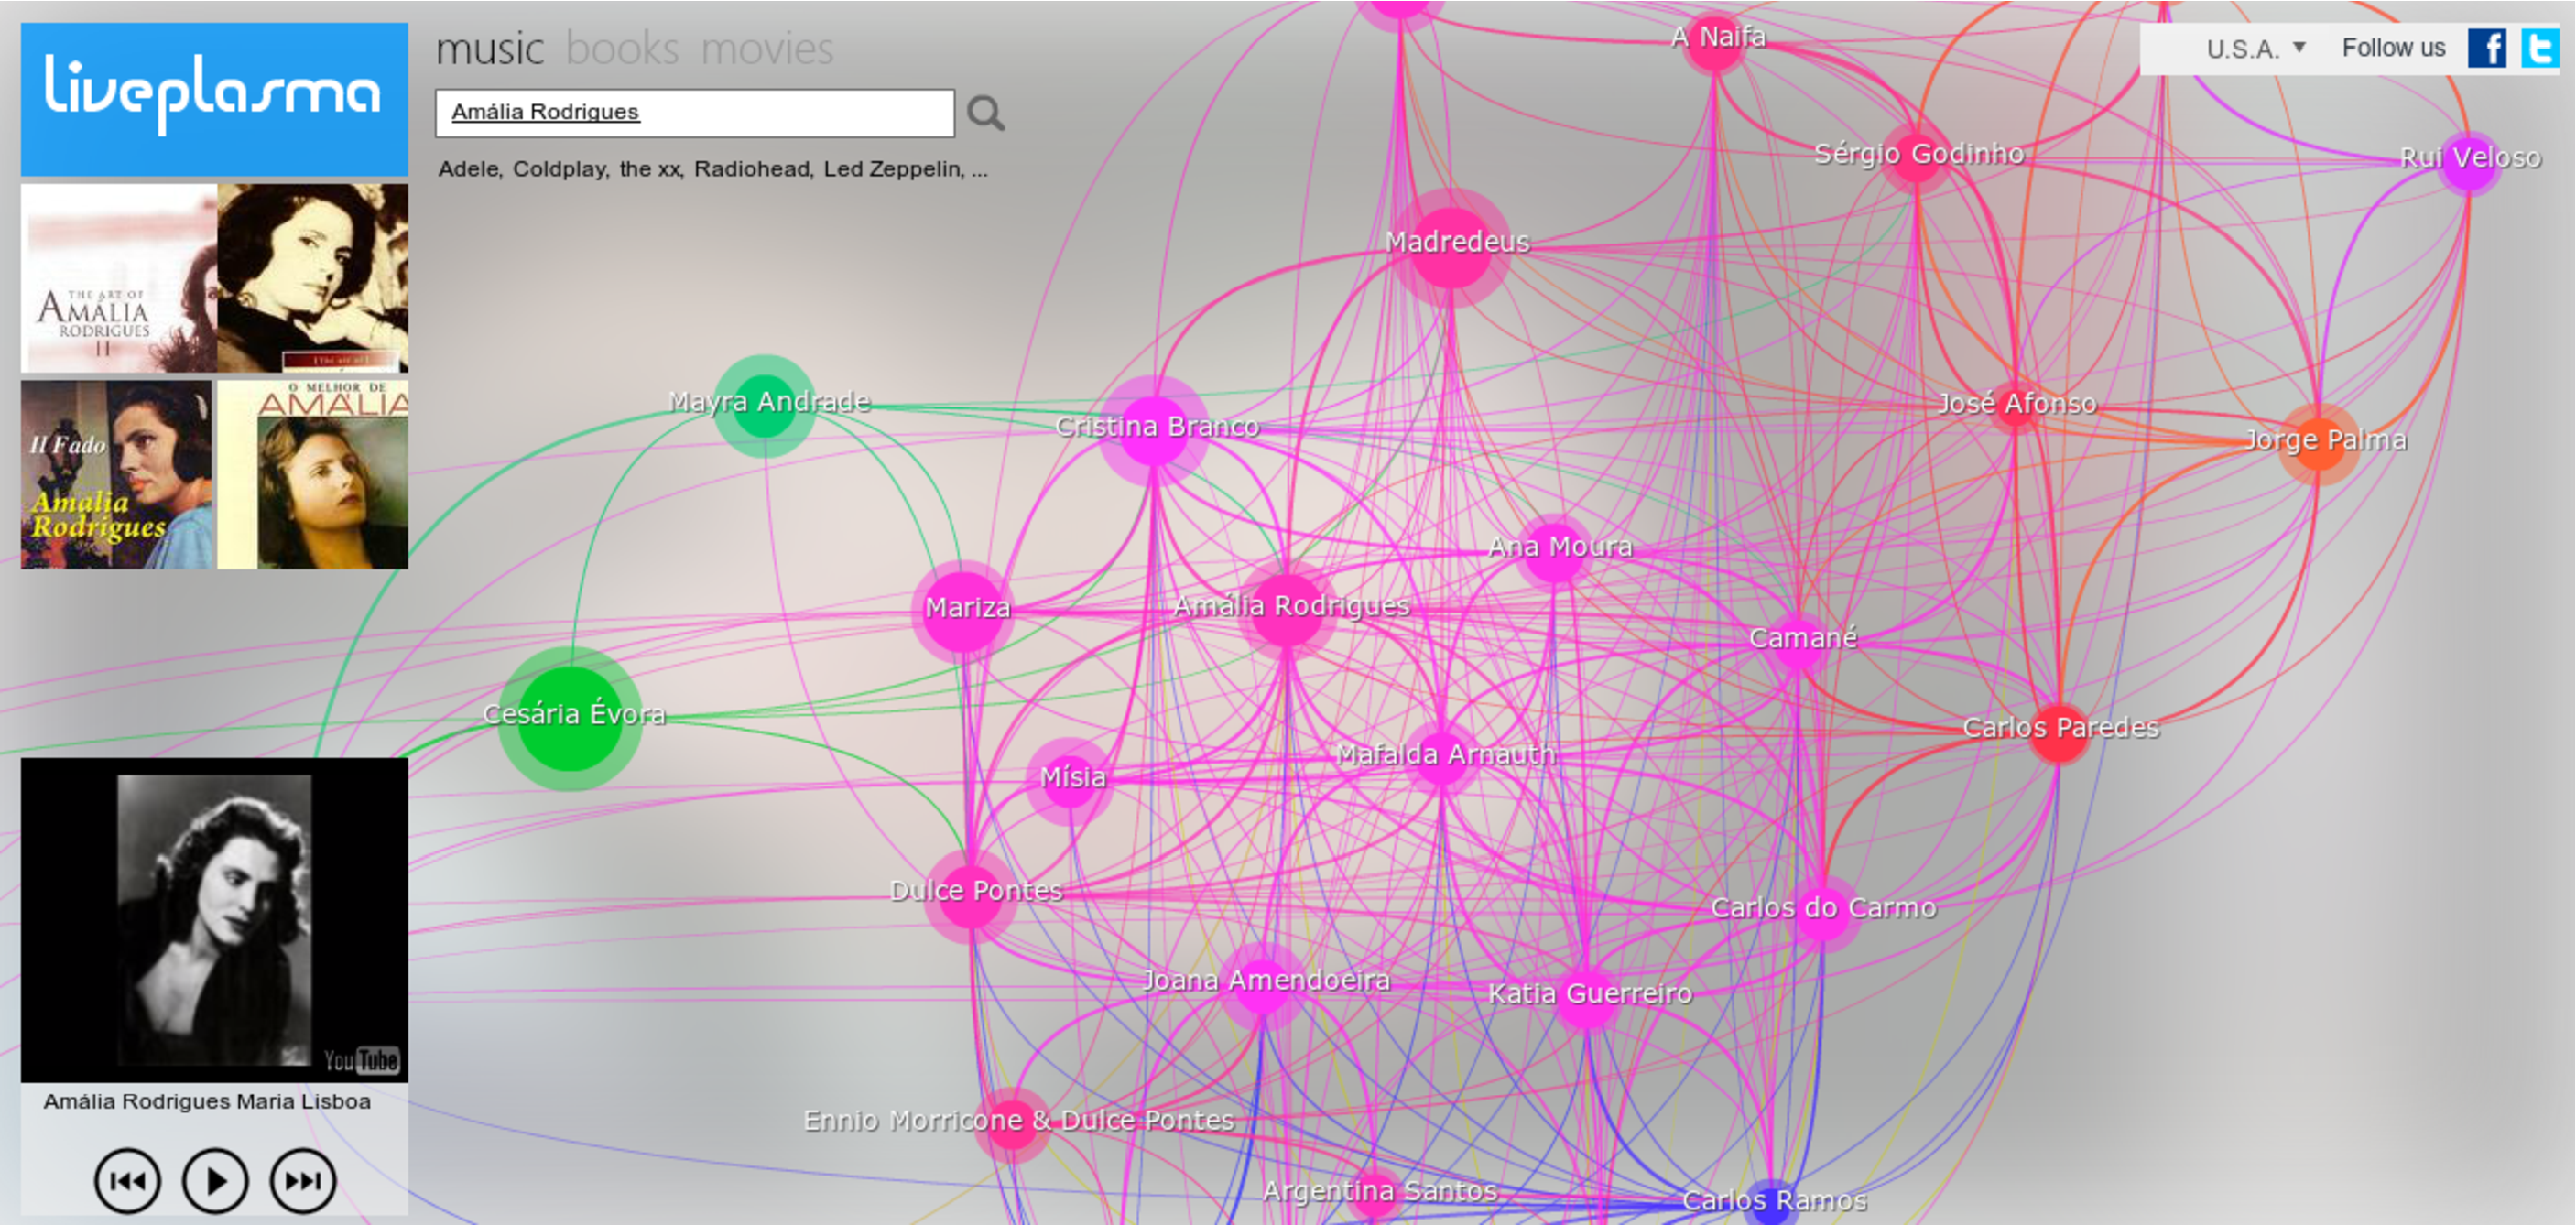
\includegraphics[width=\textwidth]{liveplasma.pdf}
  \end{center}
  \caption{liveplasma: search result for "Amália Rodrigues"; upper left corner: artist albums; lower left corner: youtube's \emph{mini-player}}
  \label{fig:sota_liveplasma}
\end{figure}

In \ref{fig:sota_liveplasma} one can see the search result for "Amália Rodrigues".

On the left side of the application there are some interesting elements: a grid of the artist's albums, a mini-player (stream from Youtube).

In \ref{fig:sota_liveplasma2} the user can have the choice to play tracks \emph{only} from that artist, or play \emph{similar} artists.

\begin{figure}[b]
  \begin{center}
    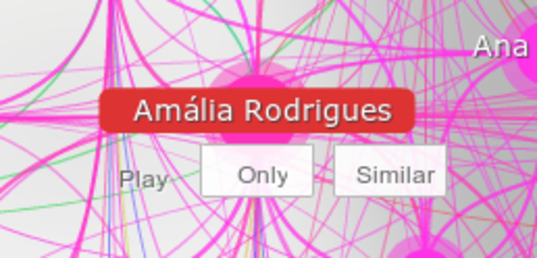
\includegraphics[]{liveplasma2.pdf}
  \end{center}
  \caption{liveplasma: interface to start playing tracks. \emph{Similar} button plays tracks from similar artists, whereas, the \emph{only} button only plays tracks from the specified artist.}
  \label{fig:sota_liveplasma2}
\end{figure}

\subsubsection{Pros} % (fold)
\label{ssub:liveplasma_pros}

This tools, has two interesting aspects to it:

\begin{itemize}
  \item Links to buy albums of the artist
  \item Play tracks from similar artists to the search artist.
\end{itemize}

% subsubsection pros (end)

\subsubsection{Cons} % (fold)
\label{ssub:liveplasma_cons}

The graph drawn from this simple search, is very cluttered with edges.
Two nodes can have several connections between, which seems to overload the graph and making it very confusing.

Different colours are used, but their meaning remains unknown. One can assume that they represent the similarity between artists, but that is just speculation.

It can also be assumed that the size of the nodes (radius value) can be directly proportional to the artist's popularity, but that is, again, just speculation.

One critical detail is that the user cannot visually point out the search node in the graph, given the lack of visual distinction from the other nodes of the graph \ref{fig:sota_liveplasma}.


% subsubsection cons (end)

\subsubsection{Summary} % (fold)
\label{ssub:liveplasma_summary}

In short, liveplasma is not very user friendly. 
It uses too many colours and edges, which makes the user experience of searching for new music even harder than usual.

% subsubsection summary (end)

% subsection liveplasma (end)

\subsection{Tuneglue - audiomap.tuneglue.net} % (fold)
\label{sub:tuneglue}

Tuneglue is another flash application that tries to explore the graphic visualization of network of related artists.
Last.fm's metadata API is used to retrieve artist information.

When you start Tuneglue and search for an artist, say "Mariza", the user is presented with a single-node graph.
By clicking the node, the user has four options (\ref{fig:sota_tuneglue}): expand, releases, lock position and delete.


\begin{figure}[bt]
  \begin{center}
    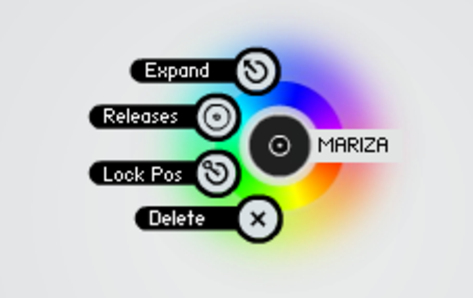
\includegraphics[]{tuneglue.pdf}
  \end{center}
  \caption{Tuneglue: menu que aparece ao clicar num nó.}
  \label{fig:sota_tuneglue}
\end{figure}

When you first expand a node, you get the root node with six child nodes \ref{fig:sota_tuneglue2}.

\begin{figure}[tb]
  \begin{center}
    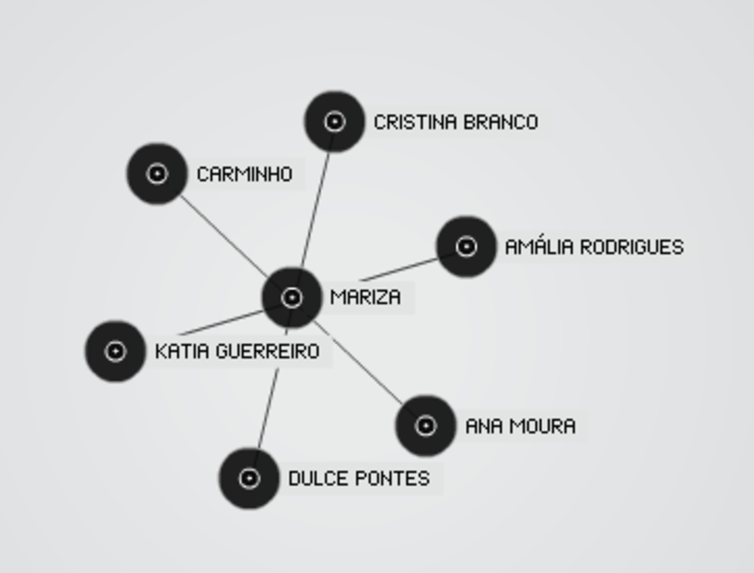
\includegraphics[]{tuneglue2.pdf}
  \end{center}
  \caption{Tuneglue: grafo depois do primeiro nó ser expandido.}
  \label{fig:sota_tuneglue2}
\end{figure}

So the first feature that brings the user experience to another level (in comparison with liveplasma) is that of graph editing.
The user can expand, fix and delete every single node in the graph.


\subsubsection{Pros} % (fold)
\label{ssub:audiomap_pros}

Tuneglue gives control to the user.
On one hand, the user is able to craft a graph and tailor it to its needs.
The user feels that graph is its own creation.

% subsubsection pros (end)

\subsubsection{Cons} % (fold)
\label{ssub:audiomap_cons}

On the other hand, the user has the responsibility to create the whole graph, which might be too much trouble and deteriorate the user experience.

Again the root node is not highlighted, which might leave the user lost when the graph gets more and more complex.

% subsubsection contras (end)

\subsubsection{Summary} % (fold)
\label{ssub:audiomap_summary}

Tuneglue takes the approach to give the user the power to create what he wants.
But with no limit, the user can easily create a very complex graph that deteriorates the user experience.


% subsubsection summary (end)

% subsection tuneglue (end)

\subsection{MusicRoamer - musicroamer.com} % (fold)
\label{sub:musicroamer}

  O MusicRoamer é outra ferramenta que permite explorar música nova.
  Tal como o Tuneglue, este permitir construir o grafo à medida que se expande cada nó.



  \subsubsection{Pros} % (fold)
  \label{ssub:pros}

  
  Umas das funcionalidades interessantes do MusicRoamer são as várias opções de pesquisa (figura~\ref{fig:sota_musicroamer}):
  \begin{description}
    \item[Pesquisa por Artista] \hfill \\
      Tipo de pesquisa mais utilizada
    \item[Pesquisa por \emph{Keyword}] \hfill \\
      Usar palavras-chave como géneros musicais para pesquisar livremente
    \item[Pesquisa por perfil do Last.fm] \hfill \\
      Esta pesquisa gera um grafo para cada artista (os mais ouvidos pelo utilizador)
  \end{description}

  \begin{figure}[tb]
    \begin{center}
      
\includegraphics[width=\textwidth]{musicroamer.pdf}
    \end{center}
    \caption{MusicRoamer: Várias opções de pesquisa. Por artista; por \emph{keyword} e pelo perfil de utilizador do Last.fm}
    \label{fig:sota_musicroamer}
  \end{figure}

  Todas estas formas de pesquisa desenham um (ou mais) grafo(s) em que os nós são sempre artistas de música.

  O que esta ferramenta trás de novo é a forma como apresenta os grafos.
  A figura~\ref{fig:sota_musicroamer3} apresenta o resultado da pesquisa por Artista "Mariza".
  Imagens dos artistas são usadas para representar os nós, o que ajuda o utilizador a diferenciar os resultados.

  A ferramenta também disponibiliza alguns parâmetros de personalização do grafo (figura~\ref{fig:sota_musicroamer2}) como Zoom, Tamanho da repulsão, imagem entre os nós e o número de artistas de música que deve expandir de um nó.

  \begin{figure}[tb]
    \begin{center}
      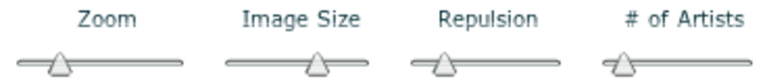
\includegraphics[width=\textwidth]{musicroamer2.pdf}
    \end{center}
    \caption{MusicRoamer: Parâmetros de personalização do grafo}
    \label{fig:sota_musicroamer2}
  \end{figure}



  \begin{figure}[tb]
    \begin{center}
      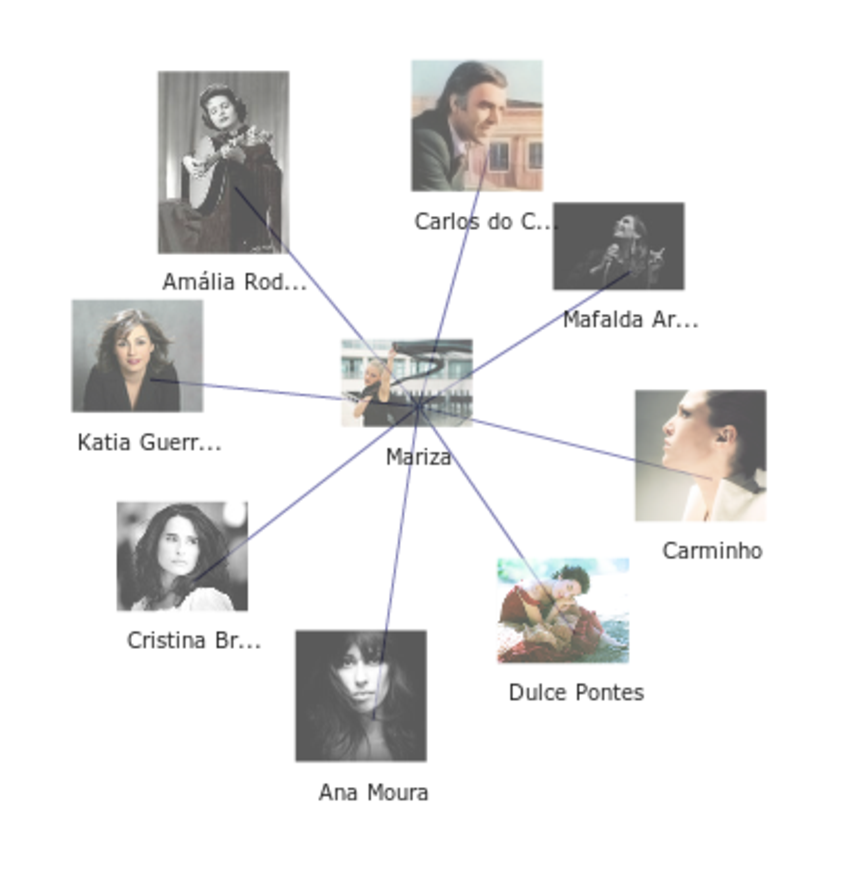
\includegraphics[width=\textwidth]{musicroamer3.pdf}
    \end{center}
    \caption{MusicRoamer: Representação visual do grafo de artistas}
    \label{fig:sota_musicroamer3}
  \end{figure}

  % subsubsection pros (end)

  \subsubsection{Cons} % (fold)
  \label{ssub:cons}

  Um problema do MusicRoamer é o facto de ser feito em flash, pois torna a interface menos natural e fluída.
  Para além disso, à medida que a profundidade do grafo vai aumentando, o grafo começa a ficar confuso e ilegível (figura~\ref{fig:sota_musicroamer4}).
  A linhas começam a se sobrepor e alguns nós ficam pouco legíveis.

  \begin{figure}[tb]
    \begin{center}
      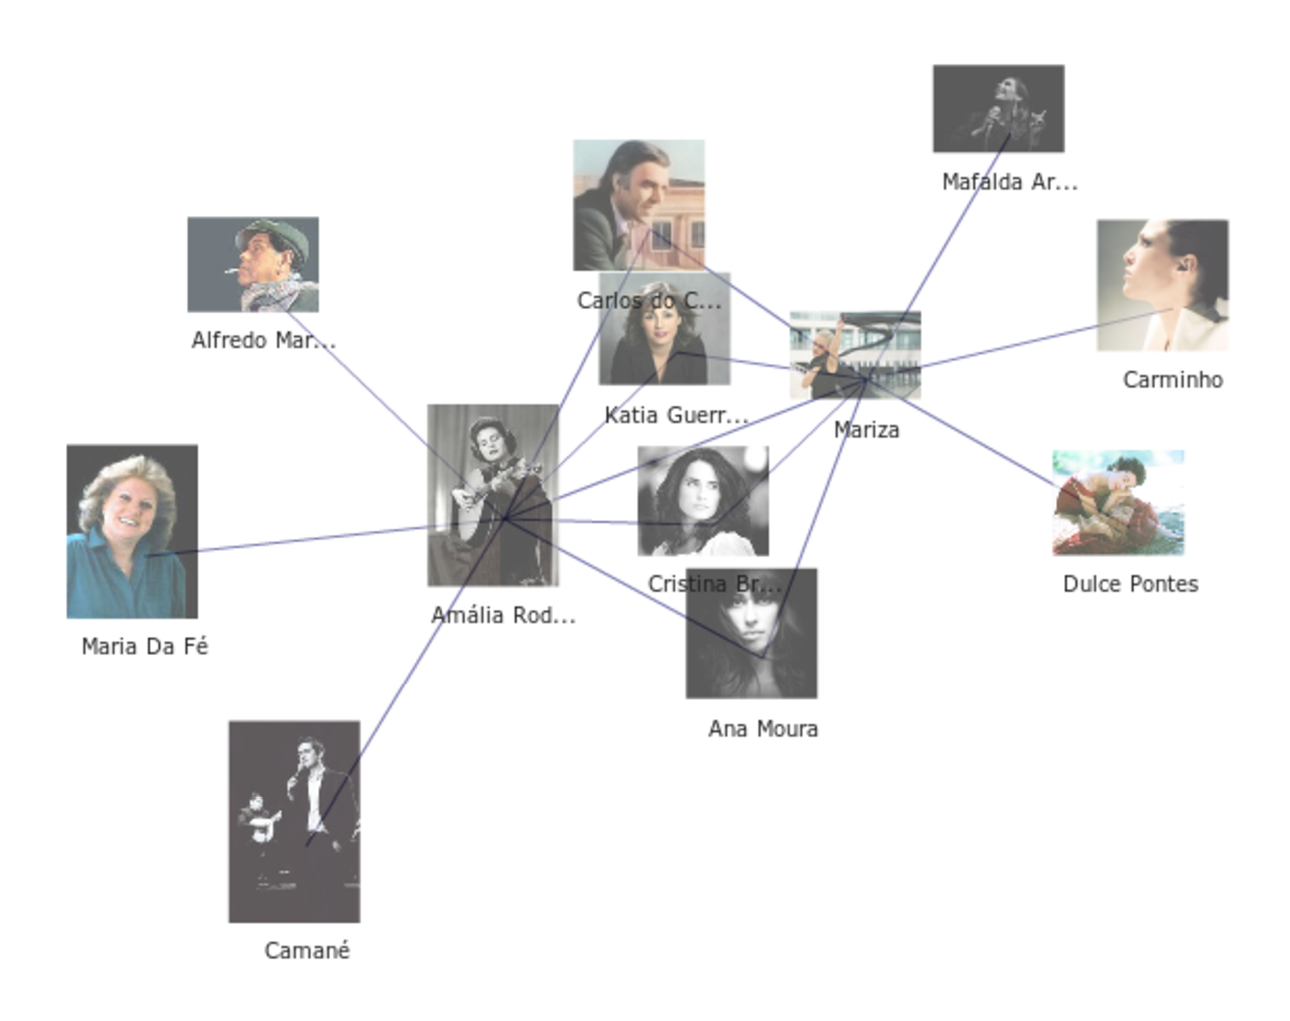
\includegraphics[width=\textwidth]{musicroamer4.pdf}
    \end{center}
    \caption{MusicRoamer: Grafo depois de expandir um nó}
    \label{fig:sota_musicroamer4}
  \end{figure}

  % subsubsection cons (end)

  \subsubsection{Summary} % (fold)
  \label{ssub:summary}

  Apesar de um utilizador do MusicRoamer ter muita liberdade na criação do grafo, a sua apresentação global é fraca e pouco trabalhada esteticamente.
  
  % subsubsection summary (end)

% subsection musicroamer (end)


% section related_similar_services (end)


\section{Conclusions}

Existem muitas outras ferramentas de descoberta de música. Apesar serem poucas as que usam esta representação visual em grafo, todas elas são importantes de se referir:

\begin{itemize}
  \item liveplasma.com
  \item audiomapa.tuneglue.net
  \item musicroamer.com
  \item discovr.info
  \item ifyoudig.net
  \item pitchfork.com
  \item hypem.com
  \item awdio.com
  \item 8tracks.com
  \item tastekid.com
  \item songza.com
  \item thesixtyone.com
  \item mog.com
  \item stereogum.com
  \item gigfi.com
  \item jango.com
  \item soundcloud.com
  \item grooveshark.com
\end{itemize}


Umas das primeiras lições que se tira dos exemplos dados é que quanto maior for o fator de ramificação de um grafo, mais confuso e saturado se torna.
Não é um exagero dizer que para além de confuso, o grafo perde o seu propósito inicial de ajudar o utilizador na sua descoberta de música nova.

Uma forma de evitar este problema, por exemplo, será limitar o fator de ramificação a um máximo que não cause este problema.